% This is samplepaper.tex, a sample chapter demonstrating the
% LLNCS macro package for Springer Computer Science proceedings;
% Version 2.20 of 2017/10/04
%
\documentclass[runningheads, anonymous=true]{llncs}
%
\let\proof\relax
\let\endproof\relax
\usepackage{graphicx}
\usepackage{hyperref}
\usepackage{amsmath}
\usepackage{amsthm}
\usepackage{amsfonts}
\usepackage{color}
\usepackage{multirow}
\usepackage{tabularx,booktabs}
\usepackage{xspace} 
\usepackage{caption}
\usepackage{subcaption}
\usepackage{enumitem}
\usepackage[table]{xcolor}
% Used for displaying a sample figure. If possible, figure files should
% be included in EPS format.
%
% If you use the hyperref package, please uncomment the following line
% to display URLs in blue roman font according to Springer's eBook style:
% \renewcommand\UrlFont{\color{blue}\rmfamily}

\newcommand{\todo}[1]{}
\renewcommand{\todo}[1]{{\color{red}{#1}}}
\newcommand{\xxx}{}
\renewcommand{\xxx}{{\texttt{\color{red}{XXX}}}\xspace}

\theoremstyle{definition}
\newtheorem{observation}[theorem]{Observation}

\begin{document}
%
\title{Beyond Chunk-Then-Embed: A Comprehensive Taxonomy and Evaluation of Document Segmentation Strategies for Information Retrieval}
%
\titlerunning{SDR for Systematic Reviews: A Reproducibility Study}
% If the paper title is too long for the running head, you can set
% an abbreviated paper title here
%

%
%\authorrunning{F. Author et al.}
% First names are abbreviated in the running head.
% If there are more than two authors, 'et al.' is used.
%

%Springer Heidelberg, Tiergartenstr. 17, 69121 Heidelberg, Germany
%\email{lncs@springer.com}\\
%\url{http://www.springer.com/gp/computer-science/lncs} \and
%ABC Institute, Rupert-Karls-University Heidelberg, Heidelberg, Germany\\
%\email{\{abc,lncs\}@uni-heidelberg.de}}
%
\maketitle              % typeset the header of the contribution
%
\begin{abstract}
%Standard: Chunk-then-embed; 
%New: Embed-then-chunk (so it's contextualised)
%For chunking: different approaches available:
%For evaluation: One-document retrieval evaluation vs multiple-document retrieval evaluatoin. 

Document chunking is a critical preprocessing step in dense retrieval systems, yet the design space of chunking strategies remains poorly understood. Recent work has proposed novel approaches ranging from LLM-guided chunking methods such as DenseX~\cite{densex2024} and LumberChunker~\cite{lumberchunker2024}, to contextualized chunking strategies like Late Chunking~\cite{latechunking2024}, which generates embeddings before segmentation to preserve contextual information. However, existing methods have been evaluated in isolation across different benchmarks, making direct comparisons difficult.

This paper presents a systematic framework that unifies existing chunking strategies along two key dimensions: (1) the \textit{order} of chunking and embedding operations (pre-embedding vs. contextualized chunking), and (2) the \textit{segmentation methods} (traditional fixed-size, sentence/paragraph-based, semantic boundary-based, and LLM-guided approaches). We reproduce and evaluate representative methods from each category across two distinct retrieval paradigms: single-document needle-in-a-haystack retrieval and multi-document web-scale retrieval.
Our comprehensive evaluation reveals that ...
%no single chunking strategy dominates across all scenarios. Contextualized chunking consistently improves retrieval quality for semantically coherent queries but incurs significant computational overhead. LLM-guided methods excel at preserving discourse structure but struggle with efficiency at scale. Fixed-size chunking, while computationally efficient, remains competitive only when chunk boundaries align with natural document structures. These findings highlight the importance of task-aware chunking strategy selection and motivate future work on adaptive chunking methods.
Our code and evaluation benchmarks are publicly available at \url{https://xx}.

%the optimal chunking strategy is highly task-dependent, with contextual methods showing substantial gains in single-document settings while pre-embedding approaches remain competitive in multi-document scenarios. We release our unified benchmark and implementations to facilitate future research in document segmentation for information retrieval.

\keywords{Chunking \and Document Ranking \and Re-ranking.}

\end{abstract}
%
%
%

\section{Introduction}
\vspace{-12pt}
A systematic review is a focused literature review that synthesises all relevant literature for a specific research topic. Identifying relevant publications for medical systematic reviews is a highly tedious and costly exercise, often involving multiple reviewers to screen (i.e., assess) upwards of tens of thousands of studies. It is a standard practice to screen each study retrieved for a systematic review by a Boolean query. However, in recent years, there has been a dramatic rise in Information Retrieval methods that attempt to re-rank this set of studies for a variety of reasons, such as stopping the screening early (once a sufficient number of studies have been found) or beginning downstream phases of the systematic review process earlier (such as the acquisition of the full-text of studies). However, a known problem with many of these methods is that they use a different query from the Boolean query used to perform the initial literature search. Instead, most methods typically resort to less informationally representative sources for queries that can be used for ranking, such as the title of the systematic review, e.g.,~\cite{miwa2014reducing} (containing narrow information about the retrieval topic), or concatenating the clauses of the Boolean query together, e.g.,~\cite{alharbi2017ranking} (negating the structural information in Boolean clauses). We instead turn our attention to methods that use more informative sources of information to perform re-ranking. 

Indeed, we focus this reproducibility study on one such method: seed-driven document ranking (SDR) from Lee and Sun~\cite{lee2018seed}. SDR exploits studies that are known a priori to develop the research focus and search strategy for the systematic review. These studies are often referred to as `seed studies' and are commonplace in the initial phases of the systematic review creation process. This method and others such as CLF~\cite{scells2020clf} (which directly uses the Boolean query for ranking) have been shown to significantly outperform other methods that use a na\"ive query representation. Despite this, the SDR method was published when there was little data for those seeking to research this topic, and there have been methods published since that did not include SDR as a comparison. To this end, we devise the following research questions (RQs) to guide our investigation into why we are interested in reproducing the SDR method:

% limitations: one dataset, single seed study


%\subsection{Research Questions}
\vspace{-8pt}
\begin{description}[leftmargin=4pt]
\item[RQ1] \textit{Does the effectiveness of SDR generalise beyond the CLEF TAR 2017 dataset?} The original study was only able to be investigated on a single dataset of systematic review topics. In this study, we plan to use our replicated implementation of SDR to examine the effectiveness of this method across more recent datasets, and datasets that are more topically varied (CLEF TAR 2017 only contains systematic reviews about diagnostic test accuracy).
%While these are indeed a challenging kind of systematic review to produce and of great importance to develop methods to assist with their creation, there are many other kinds of systematic reviews of varying difficulty to produce).
\item[RQ2] \textit{What is the impact of using multiple seed studies collectively on the effectiveness of SDR?} The original study focused on two aspects of their method: an initial ranking using a single seed study and an iterative ranking which further uses the remaining seed studies one at a time. We focus on investigating the first aspect concerning the impact of multiple seed studies (multi-SDR) used collectively for input to produce an initial ranking.
%The original study only utilised a single seed study to produce a ranking.
\item[RQ3] \textit{To what extent do seed studies impact the ranking stability of single- and multi-SDR?} 
%Finally, we examine the impact of seed studies on the variability of SDR effectiveness. 
In a recent study by Scells et al.~\cite{scells2020comparison} to generate Boolean queries from seed studies, it was found that seed studies can have a considerable and significant effect on the effectiveness of resulting queries. We perform a similar study that aims to measure the variance in effectiveness of SDR in single- and multi- seed study settings.
\end{description}

%\noindent
%With the investigation into the above research questions, we will:
%\begin{itemize}[leftmargin=*]
%\item Demonstrate the \textbf{novelty} of the method by performing experiments on more datasets (\textbf{RQ1}), and experiments that reveal more about the effectiveness of the method (\textbf{RQ2}, \textbf{RQ3}).
%\item Assess the \textbf{impact} of SDR towards the Information Retrieval community and the wider systematic review community.
%\item Investigate the \textbf{reliability} of SDR by comparing it to several baselines, including those by participants at the CLEF TAR shared tasks, on publicly available datasets.
%\item Make our complete reproduced implementation of SDR publicly \textbf{available} for others to use as a baseline in future work on re-ranking for systematic reviews.
%\end{itemize}
\noindent
With the investigation into the above research questions, we will (1) demonstrate the \textbf{novelty} of the method by performing experiments on more datasets (\textbf{RQ1}), and experiments that reveal more about the effectiveness of the method (\textbf{RQ2}, \textbf{RQ3}), (2) assess the \textbf{impact} of SDR towards the Information Retrieval community and the wider systematic review community, (3) investigate the \textbf{reliability} of SDR by comparing it to several baselines on publicly available datasets, and (4) make our complete reproduced implementation of SDR publicly \textbf{available} for others to use as a baseline in future work on re-ranking for systematic reviews.

\vspace{-12pt}
\section{Replicating SDR}
\vspace{-8pt}


%\subsection{Observations on Relevant Documents}
In the original paper of Lee and Sun, they devise two experimental settings for SDR: an initial ranking of retrieved studies using a seed study and iteratively re-ranking by updating the query used for SDR with one seed study at a time to simulate the manual screening process. We focus on the initial ranking stage for two reasons: (1) screening prioritisation is an accepted practice in the systematic review creation process as all studies must still be screened~\cite{chandler2019cochrane}; and (2) an effective initial ranking will naturally result in a more effective and efficient re-ranking of studies, as more studies that are relevant will be identified faster.
The intuition for SDR is that relevant studies are similar to each other. The original paper makes two important observations about seed studies to support this intuition: (1) that relevant studies are more similar to each other than they are to non-relevant studies; and (2) that relevant studies share many \textit{clinical terms}. These two observations are used to inform the representation and scoring of studies, given a seed study. We attempt to replicate these observations below to verify both that our implementation follows the same steps to make similar observations and whether the assumptions derived from them hold.
%
%We begin by investigating these observations about clinical terms to determine if the intuitions about using them are valid or not.

\begin{observation}
For a given systematic review, its relevant documents share higher pair-wise similarity than that of irrelevant documents.
\end{observation}

%The observation made is valid as relevant studies do share higher intra similarity compared with irrelevant documents. However, as negative studies were randomly chosen, the differences between their actual differences can only be treated as a reference, the actual comparing space for negative studies are much larger than that of positive studies, which means, higher intra-similarities with a particular seed document would always represent the study will be included definitely.
\noindent
We find that this observation is valid in our reproduction, as demonstrated by Figure~\ref{fig:replicating.pairwise-similarity}. In order to produce this plot, irrelevant studies were randomly under-sampled ten times. The number of non-relevant studies is always the same as the number of relevant studies for each topic. This means it is unlikely that we will produce the exact result initially found for this observation by Lee and Sun. Furthermore, one reason that the average pairwise similarity for the relevant studies may not match the original results is that the textual content of studies on PubMed may have changed or been updated. Rather than using a dump of PubMed from 2017, we used the latest version of studies on PubMed, as it is unknown the exact date that studies were extracted from PubMed in the original paper, and the CLEF TAR dataset does not give an exact date. 



\begin{observation}
Relevant documents for a given systematic review share high commonality in terms of clinical terms.
\end{observation}

\noindent
We found that this observation is also valid in our reproduction, as demonstrated in Figure~\ref{fig:replicating.commonality}. It can be seen that the commonality of terms for the bag of words (BOW) and bag of clinical words (BOC) representations closely match those reported by Lee and Sun. However, we also found that with some minor modifications to the pre-processing of studies, we achieved a similar (yet still lower) commonality for terms using the BOW representation. We believe that the BOC representation shares a higher commonality of terms because the vocabulary size is smaller than the BOW representation. 
Naturally, with a smaller vocabulary, it is more likely for studies to share common terms.
%When pre-processing studies using the method suggested in original paper, we obtain a vocabulary size of 1,612,974 from BOW, thus the number of distinct clinical terms extracted only count for 4.6 \% of the vocabulary, while using preprocessing of proposed method in our paper, the number of distinct clinical terms counts for 30 \% in the BOW word space. With thee same number of BOC clinical terms extracted, our method only obtain 14.75 \% of the vocabulary size in original preprocessing method. 
When pre-processing studies using the method described in original paper, we find that BOC terms count for 4.6\% of the vocabulary, while they account for 31.2\% using our pre-processing. In fact, our BOW vocabulary is only 14.8\% their BOW vocabulary. Note that BOC is a distinct subset of BOW.


\begin{figure}[t!]
	\vspace{-12pt}
	\centering
	\begin{minipage}[t]{.48\columnwidth}
		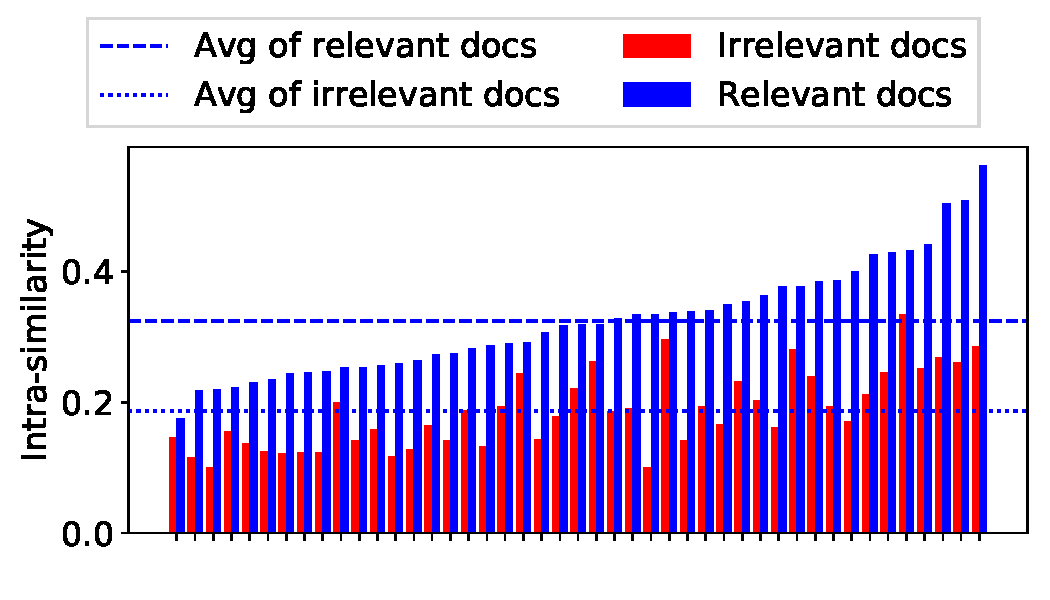
\includegraphics[width=\columnwidth]{pics/intra_sim.pdf}
		\vspace{-24pt}
		\caption{Intra-similarity between relevant studies and irrelevant studies.}
		\label{fig:replicating.pairwise-similarity}
	\end{minipage}
	\hspace{8pt}
	\begin{minipage}[t]{.48\columnwidth}
		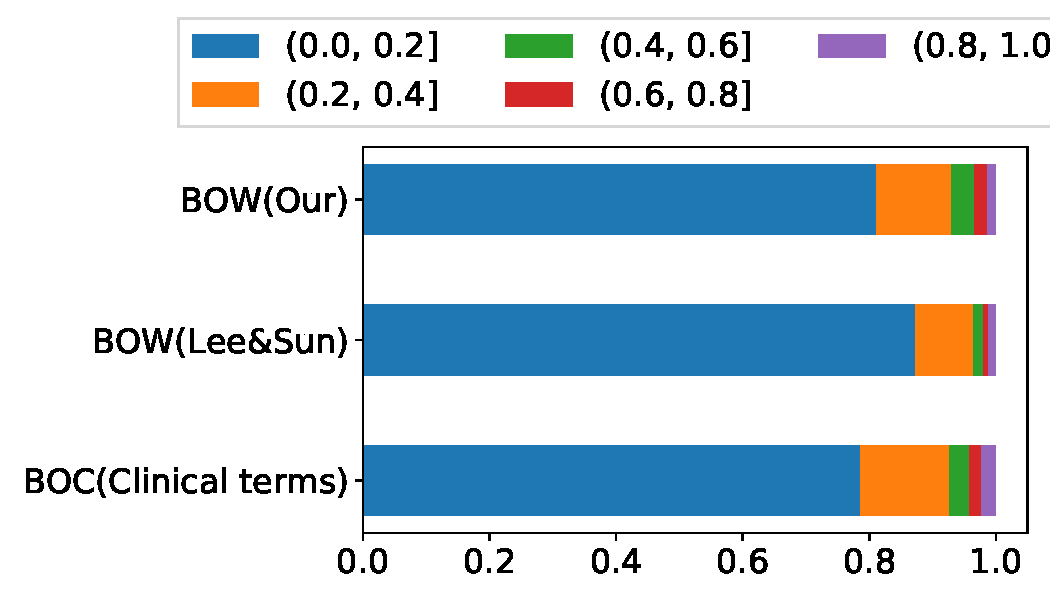
\includegraphics[width=\columnwidth]{pics/weighted1_bow_weighted1_bow_cased_lee_weighted1_boc_word.pdf}
		\vspace{-24pt}
		\caption{Distribution of terms in relevant studies.}
		\label{fig:replicating.commonality}
	\end{minipage}
	\vspace{-12pt}
\end{figure}

\vspace{-12pt}
\subsection{Document Representation}
\vspace{-4pt}

Given Observation 1 about relevant studies for this task, Lee and Sun chose to represent studies as a `bag of clinical words' (BOC). They chose to use the Unified Medical Language System (UMLS) as their ontology of clinical terms. UMLS is an umbrella ontology that combines many common medical ontologies such as SNOMED-CT and MeSH. In order to identify UMLS concepts (and therefore the clinical terms) within the studies, Lee and Sun combine the outputs of the NCBO Bioportal~\cite{noy2009bioportal} API\footnote{\url{http://data.bioontology.org/documentation}} and QuickUMLS~\cite{soldaini2016quickumls}. We follow their process as described, however we are not aware if it is not possible to set a specific version for the NCBO API. We use QuickUMLS version 1.4.0 with UMLS 2016AB.

\vspace{-12pt}
\subsection{Term Weighting}
\label{sec:replicate.term-weighting}
\vspace{-4pt}

SDR weights terms based on the intuition that terms in relevant studies are more similar to each other (or occur with each other more frequently) than non-relevant studies.
%Therefore, SDR weights terms to promote this intuition.
The weight of an individual term in a seed study is estimated by measuring to what extent it separates similar (pseudo-relevant) and dissimilar (pseudo-non-relevant) studies.
Formally, each term $t_i$ in a seed document $d_s$ ($t_i\in d_s$) is weighted using the function $\varphi (t_i,d_s) = \text{ln}\left(1+\frac{\gamma(D_{t_i},d_s)}{\gamma(D_{\bar{t_i}},d_s)}\right)$, 
%in Equation~\ref{eq:term-weight}
%\vspace{-8pt}
%\begin{equation}\label{eq:term-weight}
%	\phi (t_i,d_s) = \text{ln}\left(1+\frac{\gamma(D_{t_i},d_s)}{\gamma(D_{\bar{t_i}},d_s)}\right)
%\end{equation}
%
%\noindent
where $D_{t_i}$ represents the subset of candidate studies to be ranked where $t_i$ appears, and $D_{\bar{t_i}}$ represents the subset of candidate studies to be ranked where $t_i$ does not appear. The average similarity between studies is computed as $\gamma(D, d_s) = \frac{1}{|D|}\sum_{d_j\in D} sim(d_j, d_s)$, 
% in Equation~\ref{eq:similarity}:
%
%\vspace{-8pt}
%\begin{equation}\label{eq:similarity}
%	\gamma(D, d_s) = \frac{1}{|D|}\sum_{d_j\in D} sim(d_j, d_s)
%\end{equation}
%
%\noindent
where $sim$ is the cosine similarity between the vector representations of the candidate study $d_j$ and the seed study $d_i$. 
%In the original implementation, studies were represented as tf-idf vectors. For reproducibility purposes, we use the same representation.
We follow the original implementation and represent studies as tf-idf vectors.

\vspace{-12pt}
\subsection{Document Scoring}
\vspace{-4pt}

The original SDR implementation uses the query likelihood language model with Jelenik-Mercer smoothing for scoring studies. Typically, this ranking function is derived as indicated by QLM shown in Equation~\ref{eq:qlm-jm-sdr}, 
%
%\begin{equation}\label{eq:qlm-jm}
%	score(d,q) = \sum_{t_i\in d,q} c(t_i, q) \cdot \text{log}\left(1+\frac{1-\lambda}{\lambda}\cdot\frac{c(t_i,d)}{L_d\cdot p(t_i|\mathbb{C})}\right)
%\end{equation}
%
%\noindent
where $c(t_i, d_s)$ represents the count of a term in a seed study, $c(t_i, d)$ represents the count of a term in a candidate study, $L_d$ represents the number of terms in a study, $p(t_i|\mathbb{C})$ represents the probability of a term in a background collection, and $\lambda$ is the Jelenik-Mercer smoothing parameter.
To incorporate the term weights as described in Subsection~\ref{sec:replicate.term-weighting}, the original paper includes $\varphi$ function into the document scoring function as shown in Equation~\ref{eq:qlm-jm-sdr}:
\vspace{-8pt}
\begin{equation}\label{eq:qlm-jm-sdr}
	score(d,d_s) = \sum_{t_i\in d,d_s} 
	\overbrace{\varphi(t_i,d_s)}^\text{Term Weight}
	\cdot 
	\overbrace{c(t_i, d_s) \cdot \text{log}\left(1+\frac{1-\lambda}{\lambda}\cdot\frac{c(t_i,d)}{L_d\cdot p(t_i|\mathbb{C})}\right)}^\text{QLM}
\end{equation}

\noindent
where $p(t_i|\mathbb{C})$ is estimated using maximum likelihood estimation over the entire candidate set of studies $C$. In the original paper, when additional seed studies were ranked in the top-$k$ set of candidate seed studies (denoted as $d_{s^\prime}$), a re-ranking was initiated by expanding each $t_i$ in $d_s$ with the new terms from $d_{s^\prime}$. For our replication study, we only consider the initial ranking of candidate studies, as an abundance of baseline methods can be used as a comparison for this task. It is also arguably the most important step as a poor initial ranking will naturally result in a less effective and less efficient re-ranking.
\vspace{-12pt}
\subsection{Multi-SDR}
\vspace{-8pt}

One assumption in the original paper is that only a single seed study can be used at a time for ranking candidate studies. We propose a modification by studying the impact of using multiple seed studies collectively. In practice, it is common for Boolean queries (i.e., the search strategies used to retrieve the set of candidate studies we use for ranking) to be developed with a handful of seed studies, not just a single seed study. We hypothesise that the effectiveness of SDR will increase when multiple seed studies are used. 
%
Each relevant study must be used as a seed study for ranking, as the seed studies are not known in any of the collections we used. Therefore the average performance across topics was recorded (i.e., leave-one-out cross-validation). This study follows the methodology for the single-SDR method described in the subsections above. How we adapt single-SDR for a multi-SDR setting, and how we make this comparable to single-SDR is described as follows.
%
\vspace{-12pt}
\subsubsection{Grouping Seed Studies}
To study multi-SDR, we adopt a similar approach to the original paper; however, we instead randomly group multiple seed studies together and perform leave-one-out cross-validation over these groups. To account for any topic differences that may impact performance, we use a sliding window across the list of seed studies so that a seed study can appear in multiple groups. The number of seed studies to fill each group was chosen to be 20\% of the total seed studies. Rather than use a fixed number of seed studies, choosing different proportions simulates the use of seed studies in practice, i.e., different amounts of seed studies may be known before conducting a review. %We also ensure that topics where 20\% of the relevant studies results in a single seed study are not included.% so that our results only contain multi-SDR, and are not confounded by single-SDR results. \todo{the last sentence isn't clear to me}
%However, to account for differences in seed studies, we also shuffle the groups $k$ times and record the average performance across the $k$ shuffles. 
\vspace{-12pt}
\subsubsection{Combining Seed Studies for Multi-SDR}
The way we exploit multiple seed studies for SDR is, we believe, similar to how Lee and Sun used multiple seed studies in their relevance feedback approach to SDR. We concatenate seed studies together such that the resulting representation can be used directly with the existing single-SDR framework. We acknowledge that there may be more sophisticated approaches to exploit multi-SDR. However, we leave this as future work as it is out of the scope for this reproducibility study.

When computing term weights for multi-SDR, we also encountered computational infeasibility for large groups of seed studies. To this end, we randomly under-sampled the number of irrelevant studies to 50 each time we compute $\varphi$.
\vspace{-12pt}
\subsubsection{Comparing Single-SDR to Multi-SDR}
\label{sec:experimental-setup.comparing}

Directly comparing the results of multi-SDR to single-SDR is not possible due to the leave-one-out cross-validation style of evaluation used for single-SDR. To address this, we apply an oracle to identify the most effective single-SDR run out of all the seed studies used for a given multi-SDR run in terms of MAP. We then remove the other seed studies used in the multi-SDR run from the oracle-selected single-SDR run so that both runs share the same number of candidate studies for ranking. 
%Within each group of seed studies, we make an assumption that not all seed studies must be used for SDR. In practice, this may occur, for example, if a seed study is found to be indeed non-relevant to the topic of the systematic review when formulating the Boolean search. Therefore, we propose the following methods for selecting seed studies to be used for Multi-SDR:

%\begin{description}
%\item[Multi-All] A baseline method that does not exclude any seed studies. We use this method as a control to determine if using fewer seed studies can be more effective than using more seed studies.
%\item[Multi-Oracle] This method tries all combinations of the seed studies for SDR to identify the most effective combination. 
%\item[Multi-Diversity] This method first attempts to rank the seed studies in terms of diversity, and then takes the top-$k$ to be used in SDR, where $k$ is proportional to the number of seed studies. 
%\end{description}



















\section{Experimental Setup}

We evaluate every chunking strategy within the unified pipeline introduced in Figure~\ref{fig:chunking-embedding-pipeline}. This section first details the configuration of that pipeline and then summarizes the datasets and evaluation methodology used to assess each variant.

\subsection{Pipeline Configuration}

\subsubsection{Chunking Modules}
Each chunking strategy from Section~\ref{sec:benchmarking_document_segmentation_strategies} is instantiated with a single implementation that applies to all datasets.
\begin{itemize}
    \item \textbf{Fixed-size windows:} Documents are divided into 512-token spans with no overlap. \todo{Confirm whether overlap or stride tuning is explored.}
    \item \textbf{Paragraph boundaries:} Segments follow newline-delimited paragraphs after lightweight normalization that collapses consecutive newlines.
    \item \textbf{Sentence blocks:} We group five consecutive sentences produced by spaCy's English sentence segmenter. \todo{Verify tokenizer language model version.}
    \item \textbf{Semantic sentence chunking:} We reuse the open-source implementation described in~\ref{todo:semantic-splitting}, using jina-embeddings-v2-small-en to score adjacency and place a boundary when cosine similarity falls below the default threshold.
    \item \textbf{LumberChunker:} We prompt Gemini-1.5-Flash for GutenQA and GPT-4.1-Nano for BEIR documents, mirroring settings published in~\cite{duarte_lumberchunker_2024}. Chunk boundaries are extracted from JSON responses and aligned back to token spans.
    \item \textbf{Proposition-level chunking:} For GutenQA we cascade LumberChunker with a second GPT-4.1-Nano prompt that enumerates propositions inside each coarse segment; for BEIR we invoke the proposition prompt directly. \todo{Document prompt templates and temperature.}
\end{itemize}

Every method emits a sequence of span offsets that is consumed by the encoder modules described next.

\subsubsection{Encoder Settings}
We evaluate four encoder families (jina-embeddings-v2-small-en, jina-embeddings-v3, nomic-embed-text-v1, and multilingual-e5-base) in two modes.
\begin{itemize}
    \item \textbf{Regular encoder (pre-embedding):} Each chunk is encoded independently, and the resulting vectors are normalized and indexed.
    \item \textbf{Late encoder (contextualized):} The full document, or overlapping slices when necessary, is passed through the encoder to obtain token-level embeddings. Span offsets from the chunker are applied afterward, and chunk vectors are produced via mean pooling. \todo{Assess whether attention pooling improves stability.}
\end{itemize}

When encoders require instruction prefixes (for example, the E5 instruction token), we prepend the prefix only to the first span and append suffix tokens to the final span so that intermediate chunks correspond to contiguous document text. All encoders operate with mixed precision (FP16) on GPU unless otherwise noted. \todo{Record hardware specifications.}

\subsubsection{Retrieval Pipeline}
Chunk vectors are stored in a FAISS flat index with cosine similarity. Retrieval consists of top-$k$ dense retrieval followed by optional re-ranking when the dataset protocol requires it. For BEIR tasks we retrieve $k=100$ chunks per query and evaluate ranking directly on dense scores; for GutenQA we retrieve $k=64$ chunks and compute metrics at the chunk level. \todo{Add ablation on larger $k$ values.}

To map chunk scores back to documents we aggregate by maximum score unless the benchmark specifies passage-level evaluation. Negative sampling and index construction are performed per encoder to avoid cross-model interference.

\subsubsection{Handling Long Documents}
\label{sec:longtext}
Encoder context windows impose practical limits on segment length. In the pre-embedding setting we ensure every chunk fits within the model limit by truncating any residual tokens conservatively. For contextualized chunking we adopt the sliding-window approach from~\cite{gunther_late_2025}: long documents are split into overlapping spans that fit the model window, each span is encoded independently, and chunk boundaries are applied within the span before pooling. Prefix tokens appear only in the first span and suffix tokens only in the last to maintain alignment.

\subsection{Datasets and Evaluation}

\subsubsection{Datasets}
We consider two complementary retrieval paradigms to stress-test generalization.
\begin{itemize}
    \item \textbf{In-document retrieval} uses GutenQA~\cite{duarte_lumberchunker_2024}, which pairs long-form literary works with question-answer annotations. Each query is restricted to one source document, emphasizing fine-grained localization. \todo{Insert summary statistics for GutenQA (number of books, average length).}
    \item \textbf{In-corpus retrieval} draws on a diverse subset of BEIR corpora~\cite{thakur_beir_2021}: FiQA, ArguAna, SciDocs, TREC-COVID, GutenQA, SciFact, and NFCorpus. These collections cover financial forums, argumentative essays, scientific abstracts, and biomedical literature. \todo{Provide per-dataset document and query counts.}
\end{itemize}

All corpora are lowercased and tokenized using the default pretrained tokenizer associated with each embedding model. We preserve dataset-specific query and relevance annotations without modification.

\subsubsection{Evaluation Metrics}
We report Discounted Cumulative Gain at rank 10 (DCG@10) for GutenQA, consistent with long-context retrieval benchmarks~\cite{duarte_lumberchunker_2024}, and normalized DCG at rank 10 (nDCG@10) for BEIR datasets~\cite{latechunking2024}. DCG@10 measures the quality of the top 10 retrieved chunks by summing graded relevance values with logarithmic discounting: $\mathrm{DCG@10}=\sum_{i=1}^{10}\frac{2^{\mathrm{rel}_i}-1}{\log_2(i+1)}$, where $\mathrm{rel}_i$ is the relevance label of the chunk at rank $i$. nDCG@10 divides DCG@10 by the score of an ideal ranking, yielding a value between 0 and 1 that facilitates comparison across queries. Metrics are calculated using the official BEIR evaluation toolkit with identical relevance thresholds across models. Confidence intervals are estimated via bootstrap resampling over queries. \todo{State number of bootstrap samples.}

\begin{table}[htbp]
	\centering
	\caption{Performance comparison across different models, chunking strategies, and datasets using DCG@10 for GutenQA and nDCG@10 for other datasets (RegularEncoder)}
	\label{tab:results_regular_encoder}
	\begin{tabular}{llccccccc}
		\toprule
		Model / Chunker && \textit{document} & \textit{corpus} & \textit{corpus} & \textit{corpus} & \textit{corpus} & \textit{corpus} & \textit{corpus} \\
		&& \textbf{GutenQA} & \textbf{fiqa} & \textbf{nfcorpus} & \textbf{scifact} & \textbf{trec-covid} & \textbf{arguana} & \textbf{scidocs} \\
		\midrule
		\multirow{6}{*}{\textbf{Jina-v2}} & Paragraph & 0.3893 & 0.3347 & 0.3042 & 0.6389 & 0.6518 & 0.4682 & 0.1843 \\
		& Sentence & 0.3261 & 0.3096 & 0.2847 & 0.6548 & 0.6674 & 0.4675 & 0.1732 \\
		& Fixed-Size & 0.3889 & 0.3339 & 0.2604 & 0.6350 & 0.6437 & 0.4706 & 0.1853 \\
		& Semantic & 0.3858 & 0.3030 & 0.2746 & 0.6445 & 0.6618 & 0.4022 & 0.1760 \\
		& Lumber & 0.4782 & 0.2754 & 0.2887 & 0.6540 & 0.6456 & 0.3906 & 0.1721 \\
		& Proposition & 0.0004 & 0.2186 & 0.2995 & 0.6331 & 0.4292 & 0.3681 & 0.1436 \\
		\midrule
		\multirow{6}{*}{\textbf{Jina-v3}} & Paragraph & 0.4574 & 0.4747 & 0.3663 & 0.7247 & 0.7721 & 0.4327 & 0.1984 \\
		& Sentence & 0.3877 & 0.4333 & 0.3566 & 0.7163 & 0.7135 & 0.4256 & 0.1888 \\
		& Fixed-Size & 0.4827 & 0.4728 & 0.3596 & 0.7262 & 0.7557 & 0.4325 & 0.1985 \\
		& Semantic & 0.4105 & 0.4396 & 0.3596 & 0.7103 & 0.7474 & 0.3894 & 0.1890 \\
		& Lumber & 0.5693 & 0.4028 & 0.3534 & 0.6845 & 0.6900 & 0.3671 & 0.1797 \\
		& Proposition & 0.0013 & 0.2858 & 0.3579 & 0.6690 & --- & 0.3044 & 0.1569 \\
		\midrule
		\multirow{6}{*}{\textbf{Nomic}} & Paragraph & 0.4893 & 0.3802 & 0.3509 & 0.7047 & 0.7652 & 0.4904 & 0.1808 \\
		& Sentence & 0.4146 & 0.3620 & 0.3502 & 0.7150 & 0.7472 & 0.5084 & 0.1732 \\
		& Fixed-Size & 0.5104 & 0.3839 & 0.3492 & 0.7050 & 0.7859 & 0.4915 & 0.1812 \\
		& Semantic & 0.4274 & 0.3562 & 0.3506 & 0.7040 & 0.7431 & 0.4434 & 0.1707 \\
		& Lumber & 0.6048 & 0.3347 & 0.3513 & 0.7093 & 0.7193 & 0.4315 & 0.1673 \\
		& Proposition & 0.0016 & 0.2575 & 0.3358 & 0.6853 & 0.5580 & 0.3693 & 0.1441 \\
		\midrule
		\multirow{6}{*}{\textbf{E5-Large}} & Paragraph & 0.4663 & 0.4617 & 0.3566 & 0.7129 & 0.6634 & 0.5999 & 0.2038 \\
		& Sentence & 0.4063 & 0.4315 & 0.3583 & 0.6873 & 0.6712 & 0.5646 & 0.1836 \\
		& Fixed-Size & 0.4862 & 0.4599 & 0.3495 & 0.7078 & 0.6590 & 0.5987 & 0.2058 \\
		& Semantic & 0.3186 & 0.4173 & 0.3583 & 0.6892 & 0.6784 & 0.5540 & 0.1888 \\
		& Lumber & 0.5234 & 0.3739 & 0.3531 & 0.6748 & 0.6931 & 0.5233 & 0.1792 \\
		& Proposition & 0.0006 & 0.2522 & 0.3602 & 0.6851 & --- & 0.3163 & 0.1551 \\
		\bottomrule
	\end{tabular}
\end{table}
\vspace{-12pt}
\section{Related Work}
\vspace{-8pt}

Currently, it is a requirement for most high-quality systematic reviews to retrieve literature using a Boolean query~\cite{chandler2019cochrane,suhail2013methods}. Given that a Boolean query retrieves studies in an unordered set, it is also a requirement that all of the studies must be screened (assessed) for inclusion in the systematic review~\cite{chandler2019cochrane}. It is currently becoming more common for a ranking to be induced over this set of studies in order to begin downstream processes of the systematic review earlier~\cite{norman2019measuring}, e.g., acquiring the full-text of studies or results extraction. This ranking of studies has come to be known as `screening prioritisation', as popularised by the CLEF TAR tasks which aimed to automate these early stages of the systematic review creation pipeline~\cite{kanoulas2017clef,kanoulas2018clef,kanoulas2019clef}. As a result, in recent years there has been an uptake in Information Retrieval approaches to enable screening prioritisation~\cite{miwa2014reducing,chen2017ecnu,alharbi2017ranking,wu2018ecnu,alharbi2018retrieving,scells2017ltr,lee2018seed,lagopoulos2018learning,abualsaud2018system,zou2018technology,scells2020clf}. The vast majority of screening prioritisation use a different representation than the original Boolean query for ranking. Often, a separate query must be used to perform ranking, which may not represent the same information need as the Boolean query. Instead, the SDR method by Lee and Sun~\cite{lee2018seed} forgoes the query all together and uses studies that have a high likelihood of relevance, seed studies~\cite{suhail2013methods}, to rank the remaining studies. 
%These studies that have a high likelihood of relevance are called `seed studies', as they \textit{seed} the initial Boolean query formulation process~\cite{suhail2013methods}. 
These are studies that are known a priori to the query formulation step. The use of documents for ranking is similar to the task of query-by-document~\cite{yang2009query,lv2011learning} which has also been used extensively in domain-specific applications~\cite{kim2014diversifying,kim2014automatic,kim2015improving}. However, as Lee and Sun note, the majority of these methods try to extract key phrases or concepts from these documents to use for searching. SDR differentiates itself from these as the intuition is that the entire document is a relevance signal, rather than certain meaningful sections. Given the relatively short length of documents here (i.e., abstracts of studies), this intuition is more meaningful than other settings where the length of a document may be much longer.
\vspace{-12pt}
\section{Conclusions}
\vspace{-8pt}

We reproduced the SDR for systematic reviews method by Lee and Sun~\cite{lee2018seed} on all the available CLEF TAR datasets~\cite{kanoulas2017clef,kanoulas2018clef,kanoulas2019clef}.
%
Across all three of these datasets, we found that the 2017 and 2018 datasets share a similar trend in results than to the 2019 dataset. We believe that this is due to topical differences between the datasets and that proper tuning of SDR would result in results that better align with those seen in 2017 and 2018.
%
We also performed several pre-processing steps that revealed that the BOW representation of relevant studies could also share a relatively high commonality of terms compared to the BOC representation. Furthermore, we found that the BOC representation for SDR is generally beneficial and that term weighting generally improves the effectiveness of SDR.
%
We also found that multi-SDR was able to outperform single-SDR consistently. Our results also used an oracle to select the most effective seed studies to compare multi-SDR to single-SDR. This means that the actual gap in effectiveness between single-SDR and multi-SDR may be considerably larger.
%
Finally, in terms of the impact of seed studies on ranking stability, we found that although multi-SDR was able to achieve higher performance than single-SDR, multi-SDR generally had a higher variance in effectiveness.
%

For future work, we believe that deep learning approaches such as BERT and other transformer-based architectures will provide richer document representations that may better discriminate relevant from non-relevant studies. Finally, we believe that the technique used to sample seed studies in the original paper and this reproduction paper may overestimate the actual effectiveness. This is because a seed study is not necessarily a relevant study, and that seed studies may be discarded after the query has been formulated. For this, we suggest that a new collection is required that includes the seed studies that were originally used to formulate the Boolean query, in addition to the studies included in the analysis portion of the systematic review.

%Automating systematic reviews through screening prioritisation reduces the time it takes to create systematic reviews, resulting in improved health care delivery. 
Further investigation into SDR will continue to accelerate systematic review creation, thus increasing and improving evidence-based medicine as a whole.

\section*{Acknowledgment}


%
% ---- Bibliography ----
%
% BibTeX users should specify bibliography style 'splncs04'.
% References will then be sorted and formatted in the correct style.
%
\bibliographystyle{splncs04}
\bibliography{bibliography}
\end{document}

